\Section{Архитектура IPv6}{Лекция 9}{Игорь Смирнов}

Предпосылки развития:
\begin{MyItemize}
    \item Малое адресное пространство IPv4
    \item Неудобный формат адреса
    \item Сложная маршрутизация
    \item Низкая защищенность (нет шифрования и аутентификации)
    \item Низкая эффективность
\end{MyItemize}

\Subsection{Адресация в IPv6}

Длина адреса~--- 128 разрядов.

Общий формат адреса:

\begin{figure}[H]
  \centering
  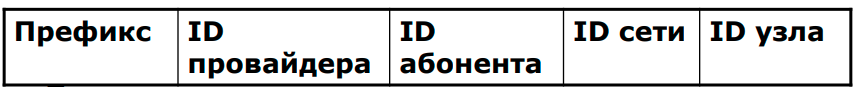
\includegraphics[width=15cm]{images/08/01}
\end{figure}

ID провайдера был вынесен отдельно, чтобы можно было междоменную маршрутизацию делать только по нему.

Типы адресов:

\begin{MyItemize}
    \item Unicast
    \begin{MyItemize}
        \item Global~--- глобальный адрес
        \item Link-local~--- адрес линии (без деления на подсети)
        \item Site-local~--- адрес узла (с делением на подсети)
    \end{MyItemize}
    \item AnyCast~--- групповой адрес, когда хотим доставить не всей группе, а кому-то одному из группы
    \item MultiCast~--- групповые адреса
\end{MyItemize}

Broadcast отсутствует.

\Subsubsection{Префикс}

\begin{MyItemize}
    \item 96 нулей~--- для совместимости с IPv4
    \item {\tt 0000 010}~--- IPX (но она умерла, поэтому не используется)
    \item {\tt 010}~--- адрес идентификации провайдера. Основной адрес, используемый в IPv6
    \item {\tt 100}~--- резервирован для географической принадлежности. е используется
    \item {\tt 1111 1110 10}~--- локальные адреса для линии
    \item {\tt 1111 1110 11}~--- локальные адреса для сети
    \item {\tt 1111 1111}~--- групповые адреса
    \item Остальные~--- резерв
\end{MyItemize}

Формат адреса идентификации провайдера:

\begin{figure}[H]
  \centering
  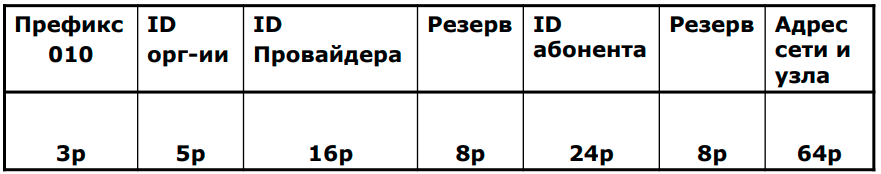
\includegraphics[width=15cm]{images/08/02}
\end{figure}

Идентификаторы организаций:
\begin{MyItemize}
    \item IANA~--- {\tt 10000}
    \item RIPE~--- {\tt 01000}
    \item INTERNIC~--- {\tt 11000}
    \item APNIC~--- {\tt 00100}
\end{MyItemize}

Это удобно для глобальной маршрутизации.

Специальные адреса:
\begin{MyItemize}
    \item Петля обратной связи (loop-back)\\
    {\tt 0:0:0:0:0:0:0:1}
    \item Не специфицированный адрес\\
    {\tt 0:0:0:0:0:0:0:0}
    \item Локальные адреса для линии\\
    {\tt 1111111010 000..000 iii.iii}\\
    Используются для адресации в локальных сегментах сетей (соединениях <<точка-точка>> и т.п.)\\
    Должны НЕ маршрутизироваться!
    \item Локальные адреса для сети\\
    {\tt 1111111011 000..000 sss..sss iii.iii}\\
    Используются для организации адресации во внутренних сетях\\
    При включении в сеть Интернет префикс может быть заменен на <<Адрес идент. провайдера>>\\
    Не должны маршрутизироваться вне данной сети
\end{MyItemize}

\Subsubsection{Anycast-адресация}

Используется для адресации <<ближайшего из группы>>. Чаще всего требуется маршрутизаторам.

Формат: <<0>> в поле идентификатора интерфейса (узла).

Anycast-адреса не могут быть адресом источника.

Anycast-адреса не могут быть приданы узлу, только маршрутизатору.

\Subsubsection{Групповая адресация}

Используется для адресации группы узлов

Формат: {\tt 11111111 000T SSSS ggg...ggggggg}

{\tt T}~--- флаг (1, если временный адрес; 0, если постоянный).

SSSS~--- атрибут видимости группы:
\begin{MyItemize}
    \item 1~--- interface-local
    \item 2~--- link-local
    \item 4~--- admin-local
    \item 5~--- site-local
    \item 8~--- organization-local
    \item 14~--- global
    \item 0, 3, 6, 7, 9-13, 15~--- зарезервированы
\end{MyItemize}

Есть предопределённые групповые адреса:
\begin{MyItemize}
    \item {\tt FF01:0:0:0:0:0:0:1} и {\tt FF02:0:0:0:0:0:0:1}~--- все узлы. Их два, так как могут быть разного scope.
    \item {\tt FF01:0:0:0:0:0:0:2}, {\tt FF02:0:0:0:0:0:0:2} и {\tt FF05:0:0:0:0:0:0:2}~--- все маршрутизаторы
    \item {\tt FF02:0:0:0:0:0:0:С}~--- DHCP-серверы
\end{MyItemize}

Групповой адрес не может являться адресом источника и не может появляться в заголовках маршрутизации.

\Subsubsection{Необходимые адреса узла}

Посмотрим на отдельный узел и отдельный маршрутизатор. У узла должны быть вот такие адреса:
\begin{MyItemize}
    \item Локальный адрес (link-local) для каждого интерфейса
    \item Присвоенные индивидуальные (unicast) адреса
    \item Петля обратной связи (loop back)
    \item Групповой адрес <<все узлы>>
    \item Групповой адрес для каждой группы, в которую входит узел
    \item ...
\end{MyItemize}

А у маршрутизатора, в дополнение к тому, что для узла:
\begin{MyItemize}
    \item Anycast-адрес <<Subnet-router>> для сети каждого интерфейса
    \item Другие Anycast-адреса, если требуются
    \item Групповой адрес <<все маршрутизаторы>>
\end{MyItemize}

\Subsection{Сетевой уровень}

Сильно отличается от IPv4, заменён почти полностью.

\Subsubsection{Заголовок}

Здесь у нас есть главный заголовок и добавочный заголовок.

Главный~--- постоянной длины, а при необходимости он расширяется цепочкой заголовков.

Формат заголовка:
\begin{MyItemize}
    \item Версия (4 бита)
    \item Приоритет (4 бита)
    \item Метка потока (24 бита)~--- чтобы маршрутизатор мог помечать только первый пакет в серии, а остальные маршрутизировать по тому же адресу
    \item Длина данных (16 бита)
    \item Следующий заголовок (8 бит)~--- аналог поля Protocol. Тут указывается, либо протокол вложенный, либо ссылка на следующий заголовок IPv6
    \item Hop limit (8 бит)~--- аналог TTL
    \item Адрес источника (128 бит)
    \item Адрес приёмника (128 бит)
    \item Данные
\end{MyItemize}

Добавления реализуются с помощью цепочки заголовков.

Разнесение функций в дополнительные заголовки:
\begin{MyItemize}
    \item Hop-by-hop options header~--- передача опций промежуточным маршрутизаторам
    \item Fragmentation header
    \item Routing header~--- маршрутизация от источника
    \item Destination options header~--- опции маршрутизации, которые касаются только последнего приёмника
    \item Authentication header (AH)
    \item Encapsulation security payload header (ESP)
\end{MyItemize}

\Subsubsection{Фрагментация}

Всегда происходит на начальном узле.

Сборка только на конечном узле.

Чтобы узнать самое узкое место на пути, используется механизм MTU path discovery process. Там по пути отсылается специальный пакет, в ответ получаем MTU. Если маршрут изменился за это время, получаем ICMP сообщение и повторяем снова.

Заголовок фрагментации:
\begin{MyItemize}
    \item Смещение
    \item Идентификатор
    \item Флаг последнего фрагмента
\end{MyItemize}

\Subsubsection{Связь со средой}

Используется аналог ARP~--- ND, NDP (Neighbour Discovery)

Заменяет ARP и помимо прочего умеет:
\begin{MyItemize}
    \item Определение адресов соседей канального уровня
    \item Определение маршрутизаторов, подсоединённых к локальной сети
    \item Получение информации о путях к соседям
    \item Получение информации о недостижимости соседей
    \item Определение параметров сети
    \item ...
\end{MyItemize}

\Subsubsection{Протокол ICMPv6}

Вместо ICMP и IGMP разработан единый протокол ICMPv6.

У него есть два типа сообщений: сообщения об ошибках и информационные сообщения.

Сообщения об ошибках:
\begin{MyItemize}
    \item Приёмник недоступен
    \item Пакет слишком большой
    \item Время истекло
    \item Ошибка параметра
\end{MyItemize}

Информационные сообщения:
\begin{MyItemize}
    \item Эхо-запрос/эхо-ответ
    \item Членство в группе
\end{MyItemize}

\Subsubsection{Маршрутизация}

Всё то же самое, что и в IPv4, кроме того, что маршрутизация от источника реализуется с помощью специального заголовка.

\Subsection{DNS}

Для прямого преобразования сделали новую ресурсную запись AAAA

Для обратного~--- так же, как и в IPv4. Сделали домен {\tt ip6.arpa}

\Subsection{Транспортный уровень}

Используются TCP, UDP и SCTP.

Переработка софта, конечно требуется (хотя бы потому, что расчёт суммы заголовка меняется).

\Subsection{Безопасность}

Реализована на основе технологии IPSEC. В IPSEC есть заголовок аутентификации AH и заголовок шифрования ESP. В IPv4 они реализованы как протоколы, а в IPv6 как заголовки. То есть безопасность есть из коробки.

\Subsection{Сосуществование стеков}

Прикладные протоколы придётся переписывать. Например, настройка прокси, параметров безопасности. Но сами протоколы не меняются.

Сейчас все ОС поддерживают IPv6, все провайдеры поддерживают, но непереход связан с тем, что это сложно сделать одновременно везде.

Сейчас есть двойные стеки протоколов. Это когда на ОС поднимаются и IPv4 и IPv6.

Есть туннелирование. Одну сеть можно использовать как транспорт для другой. На пограничных маршрутизаторах поддерживается и IPv6 и IPv4. Когда нужно что-то передать по каналу, который не поддерживает IPv6, мы заворачиваем IPv6 в IPv4 с помощью туннеля. Это замедляет передачу, но позволяет сделать её прозрачной.

Ещё есть трансляция адресов. Есть зарезервированный блок адресов в IPv6.
